\documentclass{article}
\usepackage{enumerate}
\usepackage{Sweave}
\begin{document}
\Sconcordance{concordance:Homework2.tex:Homework2.Rnw:%
1 2 1 1 0 6 1 1 2 1 0 2 1 27 0 1 5 17 1 1 2 1 0 3 1 7 0 1 2 5 1 1 2 1 0 %
4 1 21 0 2 1 3 0 1 2 11 1 1 2 1 0 1 1 8 0 1 1 4 0 1 2 16 1 1 2 1 0 1 1 %
7 0 1 2 3 1 1 2 1 0 1 1 7 0 2 2 5 0 2 2 5 0 1 2 17 1}


\begin{enumerate}

\item

\begin{Schunk}
\begin{Sinput}
> RENTS <- read.csv("~/Documents/Stat103/OFFICE RENTS.csv")
> lmRENTS<-lm(RENTS[,2]~RENTS[,1])
> summary(lmRENTS)
\end{Sinput}
\begin{Soutput}
Call:
lm(formula = RENTS[, 2] ~ RENTS[, 1])

Residuals:
    Min      1Q  Median      3Q     Max 
-5.1521 -2.2374  0.1688  1.9937  4.9807 

Coefficients:
            Estimate Std. Error t value Pr(>|t|)    
(Intercept) 20.63971    1.14279  18.061  < 2e-16 ***
RENTS[, 1]  -0.30380    0.08958  -3.391  0.00209 ** 
---
Signif. codes:  0 ‘***’ 0.001 ‘**’ 0.01 ‘*’ 0.05 ‘.’ 0.1 ‘ ’ 1

Residual standard error: 2.873 on 28 degrees of freedom
Multiple R-squared:  0.2911,	Adjusted R-squared:  0.2658 
F-statistic:  11.5 on 1 and 28 DF,  p-value: 0.002089
\end{Soutput}
\begin{Sinput}
> #plot(RENTS[,2], RENTS[,1])
> #abline(lm(RENTS[,2] ~ RENTS[,1]))
> 
\end{Sinput}
\end{Schunk}


\begin{enumerate}[a]
\item y=20.64-0.30

\item Yes, because the p value of the negative slope is 0.00209 which is far below 0.05

\item Since the coefficient of determination is .2911, it appears the data fits fairly poorly. Only 29.11\% of the variation in Y is explained by the model.

\item The coefficient $\hat{\beta} _1$ represents the estimated slope of the regression line. For every one percent increase in vacancy we predict a mean decrease of $\hat{\beta} _1$ = 0.30 increase in dollars per square foot of rent. 

\item 
Typically we cannot interpret $\hat{\beta} _0$ because we do no typically measure the predictor at 0, thus the value of this intercept is extrapolated. If we do measure at or very close to x=0, then we may interpret $\hat{\beta} _0$ as $\hat{y}$ when x=0. In this example interpreting $\hat{\beta} _0$ would be extrapolation.

\item Prior to using this model we must check the two assumptions made by the model. The first is that the error, $\epsilon$ is normally distributed with mean 0 and constant standard deviation. We also assumed that the residuals are independent of eachother

\item

\begin{Schunk}
\begin{Sinput}
> RentValue <- RENTS$Rent
> Vacancy <- RENTS$Vacancy
> value<-data.frame(Vacancy = 12)
> predict(lm(RentValue~Vacancy), value, level = .90, interval = "confidence")
\end{Sinput}
\begin{Soutput}
       fit    lwr      upr
1 16.99413 16.096 17.89227
\end{Soutput}
\end{Schunk}
So we may predict with 90\% confidence the the average price of rent in a city with a 12\% vacancy rate is between 16.1 dollars per square foot and 17.9 dollars per square foot.
\end{enumerate}
\item

\begin{enumerate}[a]
\item 
\begin{Schunk}
\begin{Sinput}
> FordTaurus <- read.csv("~/Documents/Stat103/FordTaurus.csv")
> Price <- FordTaurus$Price
> Odometer <- FordTaurus$Odometer
> lmFORD <- lm(Price~Odometer)
> summary(lmFORD)
\end{Sinput}
\begin{Soutput}
Call:
lm(formula = Price ~ Odometer)

Residuals:
    Min      1Q  Median      3Q     Max 
-365.16 -117.51    0.65   93.87  345.62 

Coefficients:
              Estimate Std. Error t value Pr(>|t|)    
(Intercept)  6.533e+03  8.451e+01   77.31   <2e-16 ***
Odometer    -3.116e-02  2.309e-03  -13.49   <2e-16 ***
---
Signif. codes:  0 ‘***’ 0.001 ‘**’ 0.01 ‘*’ 0.05 ‘.’ 0.1 ‘ ’ 1

Residual standard error: 151.6 on 98 degrees of freedom
Multiple R-squared:  0.6501,	Adjusted R-squared:  0.6466 
F-statistic: 182.1 on 1 and 98 DF,  p-value: < 2.2e-16
\end{Soutput}
\begin{Sinput}
> plot(Odometer,Price)
> abline(lmFORD)
\end{Sinput}
\end{Schunk}



There does appear to be a linear relationship between odometer reading and resale price. The t-value of the slope is very small, -13.49, indicating the slope is not zero. There appears to be a strong linear relationship because the correlation coefficient is 65.01$\%$

\item 

$\hat{y}$ = 6533 - 0.0311*x

\item The two assumptions about the error variable are the $\epsilon$ is normally distributed with mean 0 and constant standard deviation, and the residuals are independent.

\item
\begin{Schunk}
\begin{Sinput}
> residualsFORD<-residuals(lmFORD)
> shapiro.test(residualsFORD)
\end{Sinput}
\begin{Soutput}
	Shapiro-Wilk normality test

data:  residualsFORD
W = 0.9919, p-value = 0.812
\end{Soutput}
\begin{Sinput}
> plot(lmFORD, which = 1)
\end{Sinput}
\end{Schunk}
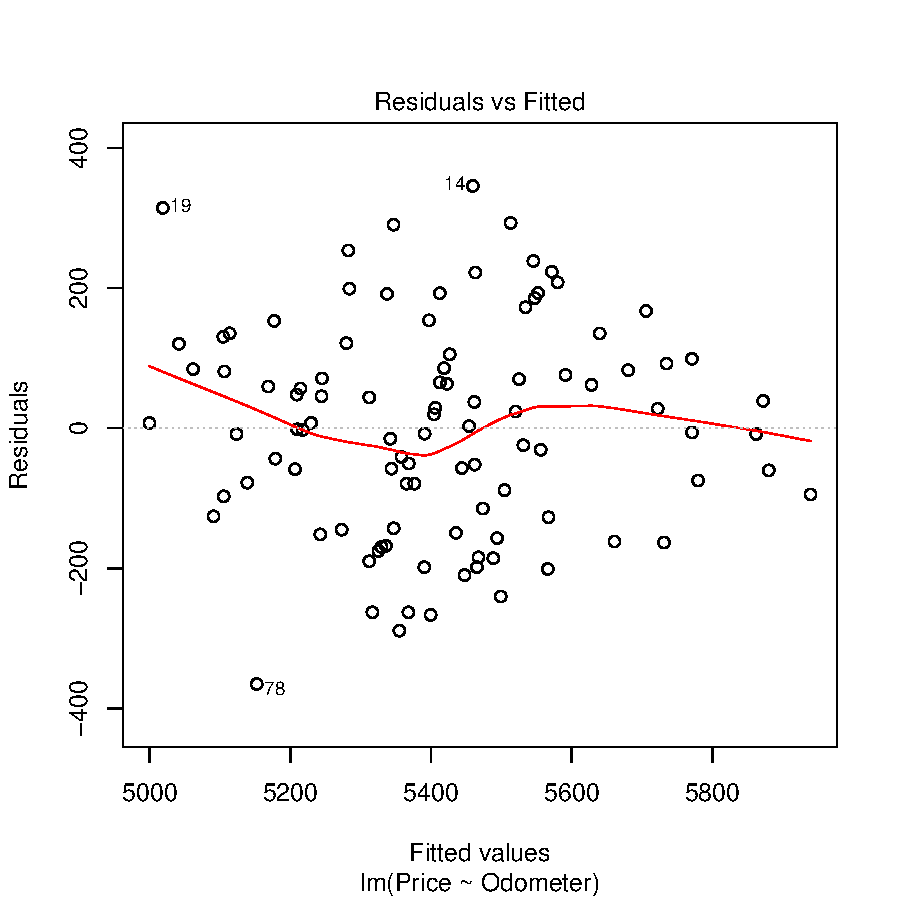
\includegraphics{Homework2-004}

I would determine the assumptions in part c are satisfied. Since the null hypothesis of the Shapiro-Wilk test for normality is that the residuals are normally distributed, a high p-value of 0.812 indicated that it is very likely the residuals are normally distributed. Upon inspecting the plot of the fitted y values and the residuals, it appears the variance of the residuals is more or less constant. There is a little tapering to the right, but is does not seem significant. 

\item From the multiple r-squared we see that 65.01\% of the variation in the resale price is explained by the regression. 

\item The coefficient $\hat{\beta} _0$=6533 extrapolates that a three year old Ford Taurus that has driven 0 miles will be resold for \$6533, but we do not interpret this because it is extrapolation. The coefficient $\hat{\beta} _1$=-0.03116 indicated that for every 100 additional miles on the odometer, we predict an average decrease of \$3.12 in resale price.

\item

$\indent$ i)The numberical value of $S_{\epsilon}$ for the model is 151.6

$\indent$ ii)The proper units for $S_{\epsilon}$ are dollars

$\indent$ iii) We interpret $S_{\epsilon}$ as the estimator for the standard deviation of the residuals. 

\item 

\begin{Schunk}
\begin{Sinput}
> car <- data.frame(Odometer = 36000)
> predict(lmFORD, car, interval = "confidence", level = .95)
\end{Sinput}
\begin{Soutput}
       fit      lwr      upr
1 5411.704 5381.626 5441.783
\end{Soutput}
\end{Schunk}
I would expect, with 95\% confidence to sell my Taurus with 36,000 miles on it for between \$5382 and \$5442.

\item

\begin{Schunk}
\begin{Sinput}
> plot<-boxplot.default(FordTaurus)
> plot$out
\end{Sinput}
\begin{Soutput}
[1] 19057
\end{Soutput}
\end{Schunk}
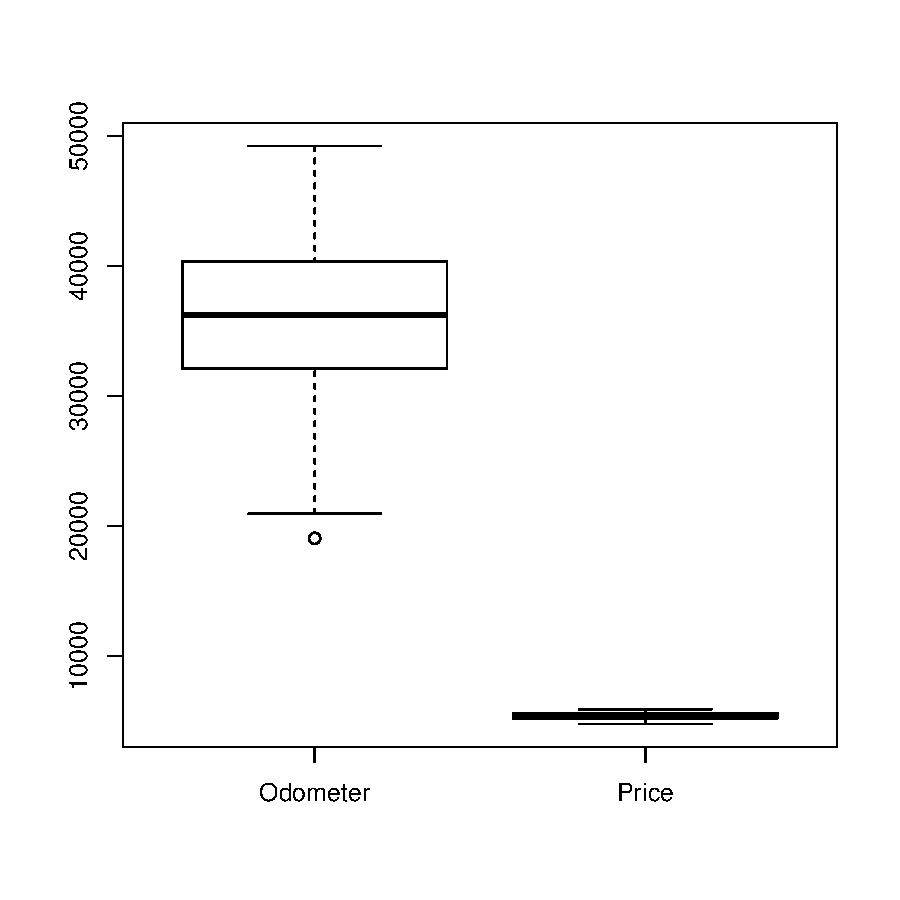
\includegraphics{Homework2-006}

\begin{Schunk}
\begin{Sinput}
> plot(lmFORD,which=5)
\end{Sinput}
\end{Schunk}
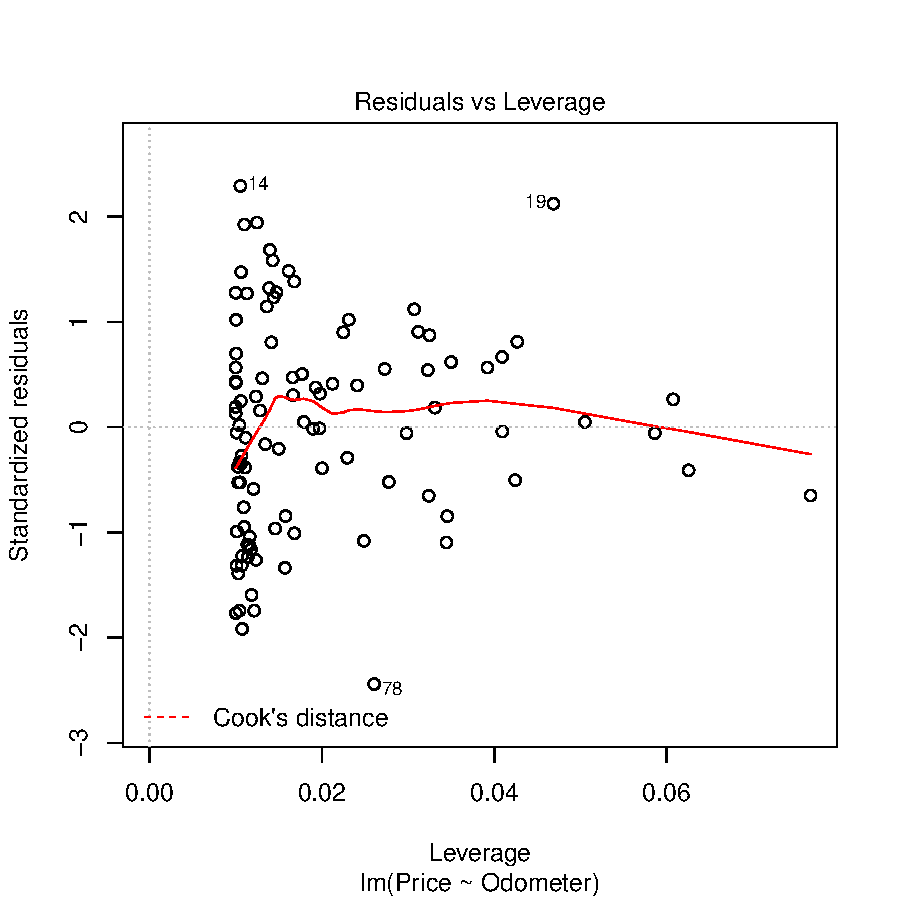
\includegraphics{Homework2-007}

\begin{Schunk}
\begin{Sinput}
> plot(lmFORD,which = 4)
\end{Sinput}
\end{Schunk}
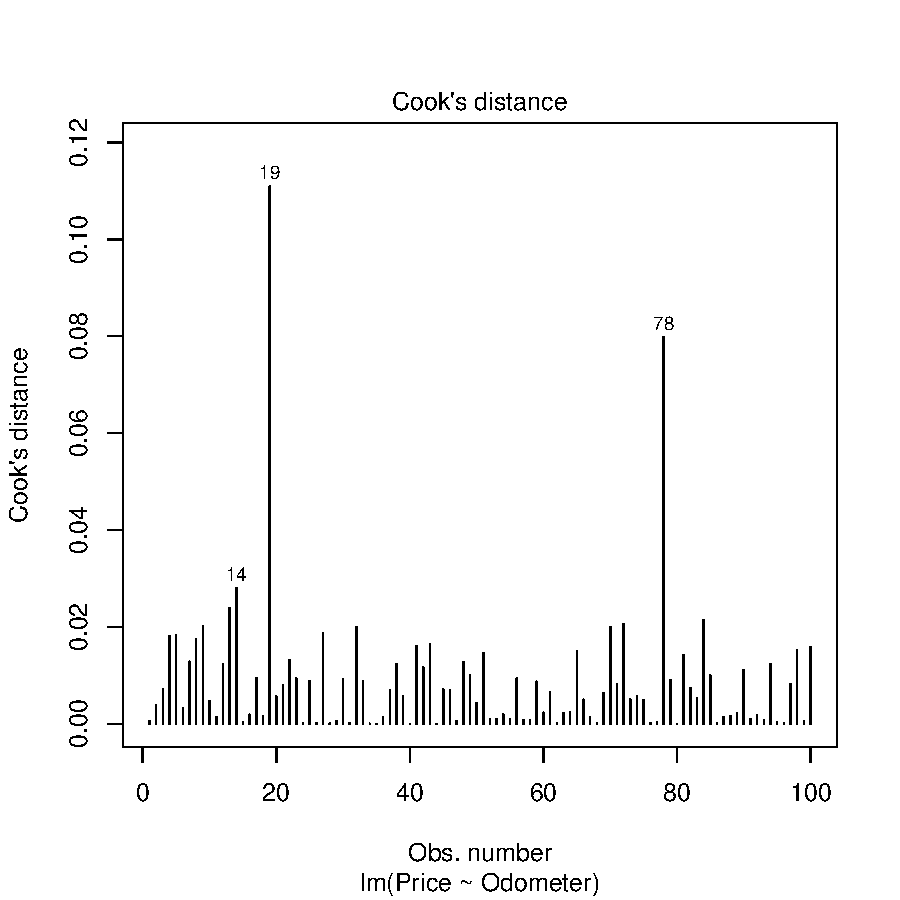
\includegraphics{Homework2-008}

I have not figured out how to find which points actuall have high leverage with R.
The influeantial point by box plot is row 8, ODO 19057, Price \$5939.61.
The potential outliers are rows 14, 19, and 78
\item

Leverage is the measure of how influential a single point is on the regression line. It is measured for each point by removing the point and observing how much it changes the slope of the regression line. Finding points with high leverage is important for finding potential outliers that lie close to the regression line.
\end{enumerate}

\item

$H_0$: $\beta _1$ = 0

$H_A$: $\mu$ $\neq$ 0

We conclude X and Y are not linearly related if we fail to reject $H_0$.
\end{enumerate}
\end{document}
